\section{Spectral Difference Method}

This section is a brief description of the space and time discretization approaches used in the present work. A more elaborated overview can be found in Refs.\ \cite{SD_I:06, SD_II:07, SD_May:06, KrisVanDenAbeele2009, Moreira2016}. %\citet{}

% Representing the continuous as a discrete
In order to represent the continuous domain of a simulation, sub-domains of the space named cells can be defined and related altogether as a contiguous set of cells named as mesh. The procedure to break down the continuous space and determine how the cells are referenced in the mesh is essential for the solver perspective. In fact, it not only determines how the data can be accessed throughout the simulation, but also how accurate a simulation can be and which kind of physical phenomena it will be capable to represent within the discrete approximation of the space. 

In general, the finer a mesh is the higher the resolution of the numerical solution, in particular when discontinuities are presented. Nonetheless, finer meshes can drastically increase the computational cost of the simulation and despite the improvements in the physical representation it may be unfeasible for real applications. 
% What is high-order method?
% Why high-order methods?

\subsection{Discretization}

The space discretization procedure of the governing equations throughout all simulations in this work is made by a high-order Spectral Difference method (SD) \cite{SD_II:07, Moreira2016}. The formulation can properly handle quadrilateral cells given an arbitrary solution accuracy order in an efficient manner by transforming each cell from its physical $x,y$ domain into a particular computational $\xi, \eta$ domain over the interval $[-1, 1]$ allowing high-order solution interpolation as presented in Refs.\ \cite{SD_II:07, SD_May:06}. The governing equations in the physical space are then transformed into the computational space and rewritten as
%
\begin{equation}
\frac{\partial \tilde{Q}}{\partial t} + \frac{\partial \tilde{F}}{\partial \xi} +
                                        \frac{\partial \tilde{G}}{\partial \eta}  = 0
\mbox{ ,}
\end{equation}
%
or in its divergence form as
%
\begin{equation}
\frac{\partial \tilde{Q}}{\partial t} + \nabla_{\xi,\eta} \cdot \tilde{\textbf{F}}  = 0
\mbox{ .}
\end{equation}
%
where the conservative variables in the computational space are defined by $\tilde{Q} = |J| \, Q$, the flux vector $\tilde{\textbf{F}} = |J|{[J]}^{-1}\textbf{F}$, $\textbf{F}$ is flux vector in the physical space,
and $J$ is the Jacobian matrix of the coordinate transformation given by
%
\begin{equation}
J = \left( \begin{array}{cc} x_\xi & x_\eta \\ y_\xi & y_\eta \end{array} \right)
\mbox{ .}
\end{equation}
%

\subsection{Space Transformation}

The coordinate transformation permits a high-order quadrilateral representation for curved boundaries by considering $N$ equally spaced nodes in the quadrilateral computational space to construct the space transformation Jacobian matrix. The space projection from the physical to the computational space for each quadrilateral can be computed by
%
\begin{equation}
    \label{eq_ho_quad_x}
    x(\xi, \eta) = \sum_{m=1}^{(N+1)^{2}}{L^{N+1}_m(\xi) L^{N+1}_m(\eta) x_{m}}
\end{equation}
%
\begin{equation}
    \label{eq_ho_quad_y}
    y(\xi, \eta) = \sum_{m=1}^{(N+1)^{2}}{L^{N+1}_m(\xi) L^{N+1}_m(\eta) y_{m}}    
\end{equation}
%
where $m$ goes through all nodes of a N-th order quadrilateral and $L^{N+1}$ is the (N+1)-th order Lagrange polynomial basis, i.e,
%
\begin{equation}
    \label{eq_lagrange}
    L^{N+1}_m(\xi) = \prod_{k=1, k \ne m}^{N+1}{\frac{(\xi-\xi_k)}{(\xi_m-\xi_k)}}
    \mbox{ .}
\end{equation}
%

\subsection{Base Polynomials}

Furthermore, two sets of intra-cell grid points are allocated, named as solution points (SP) and flux points (FP). 
The former set storages the nodal values of the conserved variables $Q$ and are located at the Gauss-Legendre quadrature points. 
The latter storages the nodal values of the flux vectors $F$ and $G$ splitted in two flux point groups 
located at a combination of the Gauss-Legendre and Gauss-Legendre-Lobatto roots to achieve a stable method according to Ref.\ \cite{KrisVanDenAbeele2009, Sun2007}. Figure\ \ref{fig:sp_fp_quad} illustrates the cell 
domain transformation as well as the intra cell grid disposal.
%
\begin{figure}[htb!]
	\centering
		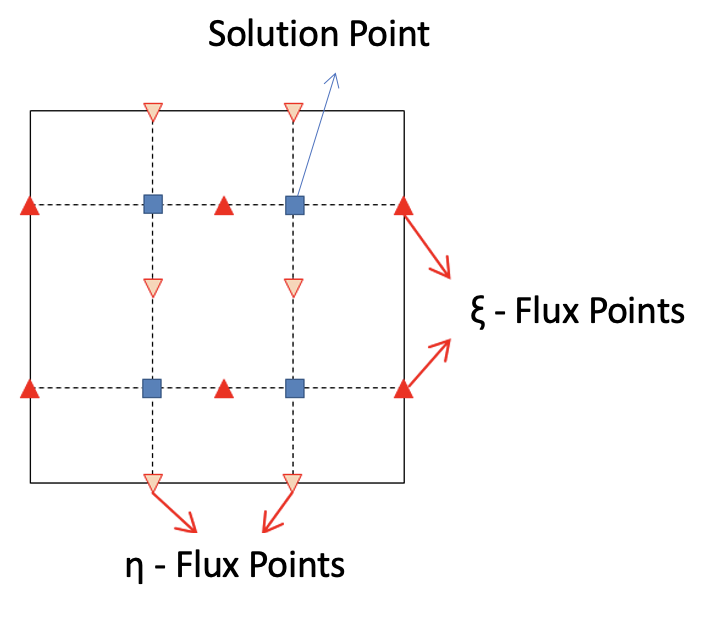
\includegraphics[height=5.0cm]{figs/sd/sp_fp_quad.png}

\caption{Quadrilateral in computational space for 2nd-order Spectral Differences, $p=1$.}
\label{fig:sp_fp_quad}
\end{figure}

The conserved solution can then be constructed at any target position within the cell computational domain by 
a nodal interpolation using a Lagrange polynomial basis as
%
\begin{equation}
    \label{eq_sp_lagr}
    {\tilde{Q}_i}(\xi, \eta) = \sum_{j=1}^{N_p}{L^{p}_j(\xi) L^{p}_j(\eta) \tilde{Q}_{i,j}}
    \mbox{ .}
\end{equation}
%
where $i$ is the i-th cell index, $j$ the j-th solution point at the i-th cell, $N_p$ the number of basis functions
required to construct a $p$ order of the polynomial interpolation, and $L^{p}$ is the p-th order Lagrange polynomial basis.

%\subsection{Numerical Imposition of Boundary Conditions}
%
%\subsubsection{Slip Wall}
%The slip wall boundary condition is applied 
%\subsubsection{Inlet}
%\subsubsection{Outlet}
%\subsubsection{Non-Reflective Farfield}
%\subsubsection{Analytical Solution}

\section{Riemann Solver}
%\subsection{Riemann Problem}
The solution vector $\textbf{Q}$ at the flux points is computed through an interpolation by Eq.\ \ref{eq_sp_lagr} and since its value is only contiguous within the cell domain, solution discontinuities at the cell interfaces can emerge during the simulation. Hence, the normal flux at the edges flux points is then reconstructed through a Riemann solver, which for all simulations of this work used a Roe scheme \cite{Roe1981}. Since only the normal component can affect the conservation properties through the cells interface, the tangential part of the flux is averaged. The basic formulation for the flux reconstruction can be written as 
%
\begin{equation}
    \label{eq_riemann}
    \tilde{F}_n = \frac{1}{2}\{(\tilde{F}_R + \tilde{F}_L) \cdot \textbf{n} - |A| (\tilde{Q}_R - \tilde{Q}_L)\}
    \mbox{ .}
\end{equation}
%
where $L$ and $R$ subscripts represent  respectively the left and right cells of an edge and $|A|$ is a representation of 
the Jacobian matrix of the flux vector which for Roe scheme is assumed to be constant between the two cells at the interface. The Roe matrix $|A_{Roe}|$ is

\begin{align} \label{eq:eq_roe_matrix}
\begin{bmatrix}
    0 & n_x & n_y & 0\\
	(\gamma - 1)\tilde{e}_k n_x - \tilde{u}_x \tilde{u}_n & \tilde{u}_n - (\gamma-2)\tilde{u}_x n_x & \tilde{u}_x n_y - (\gamma-1)\tilde{u}_y n_x & (\gamma-1)n_x\\
	(\gamma - 1)\tilde{e}_k n_y - \tilde{u}_y \tilde{u}_n & \tilde{u}_y n_x - (\gamma-1)\tilde{u}_x n_y & \tilde{u}_n - (\gamma-2)\tilde{u}_y n_y & (\gamma-1)n_y\\
	[(\gamma - 1)\tilde{e}_k -\tilde{h}]\tilde{u}_n & \tilde{h}n_x - (\gamma-1)\tilde{u}_x \tilde{u}_n & \tilde{h}n_y - (\gamma-1)\tilde{u}_y \tilde{u}_n & \gamma\tilde{u}_n
\end{bmatrix}     
\end{align}
where $n_x$ and $n_y$ are the components of the unit normal vector $n$. The properties are Roe-averaged values which can be defined through the left $L$ and right $R$ states at the interface as

\begin{equation}
    \label{eq_roe_density}
    \tilde{\rho} = \sqrt{\rho_L}\sqrt{\rho_R},
\end{equation}
%
\begin{equation}
    \label{eq_roe_ux}
    \tilde{u}_x = \frac{u_L \sqrt{\rho_L} + u_R \sqrt{\rho_R}}{\tilde{\rho}},
\end{equation}
%
\begin{equation}
    \label{eq_roe_uy}
    \tilde{u}_y = \frac{v_L \sqrt{\rho_L} + v_R \sqrt{\rho_R}}{\tilde{\rho}},
\end{equation}
%
\begin{equation}
    \label{eq_roe_ek}
    \tilde{e}_k = \frac{{\tilde{u}_x}^2 + {\tilde{u}_y}^2}{2},
\end{equation}
%
\begin{equation}
    \label{eq_roe_un}
    \tilde{u}_n =\tilde{u}_x n_x + \tilde{u}_y n_y,
\end{equation}
%
\begin{equation}
    \label{eq_roe_h}
    \tilde{h} = \frac{h_L \sqrt{\rho_L} + h_R \sqrt{\rho_R}}{\tilde{\rho}},
\end{equation}

The Roe scheme considers the characteristics decomposition, {\em i.e.}, the decomposition of the Roe matrix into waves and, then, a diagonalization of the matrix is provided such that $|A_{Roe}| = T|\Lambda|T^{-1}$. Equation\ \ref{eq_riemann} can be rewritten as
%
\begin{equation}
    \label{eq_riemann_roe}
    {\tilde{F}_{Roe_n}} = \frac{1}{2}\{(\tilde{F}_R + \tilde{F}_L) \cdot \textbf{n} - T|\Lambda| T^{-1} (\tilde{Q}_R - \tilde{Q}_L)\}
    \mbox{ .}
\end{equation}
where the matrices $T$ and $T^{-1}$ represent the eigenvectors and $\Lambda$, a diagonal matrix with the Roe eigenvalues given by
%
\begin{equation}
    \label{eq_roe_l1}
    \tilde{\lambda_{1}} = \tilde{u}_n ,
\end{equation}
%
\begin{equation}
    \label{eq_roe_l2}
    \tilde{\lambda_{2}} = \tilde{u}_n ,
\end{equation}
%
\begin{equation}
    \label{eq_roe_l3}
    \tilde{\lambda_{3}} = \tilde{u}_n +\tilde{c},
\end{equation}
%
\begin{equation}
    \label{eq_roe_l4}
    \tilde{\lambda_{4}} = \tilde{u}_n -\tilde{c},
\end{equation}
where $\tilde{c} = \sqrt{(\gamma-1)(\tilde{h}-\tilde{e}_k )}$. From Eq.\ \ref{eq_riemann_roe}, the $\tilde{\lambda}_{\ell}$ eingenvalues are the wave speeds of the approximate Riemann problem, while the characteristic variables represents the wave amplitudes which can be determined by 
%
\begin{equation}
    \label{eq_w_char_val}
    W = T^{-1}\tilde{Q}
    \mbox{ .}
\end{equation}
%
therefore, the Roe scheme applied to the second term of Eq.\ \ref{eq_riemann} becomes
%
\begin{equation}
    \label{eq_roe_piece}
    T\Lambda (W_R - W_L) = \sum_{k=1}^{m}{\tilde{\alpha}_i |\lambda_i|\tilde{T}^{(k)}}
    \mbox{ .}
\end{equation}
%
where $\tilde{\alpha}_i$ are the wave strength parameters obtained by projecting the jump in the characteristics properties $\Delta W = (W_R - W_L)$ onto the $T$ eigenvector. The projected matrix represented by $\tilde{T}$ can be defined as
\begin{equation}
    \label{eq_t_projected}
	\tilde{T} = 
\begin{bmatrix}
    1 & 0 & 1 & 1\\
    \tilde{u}_x & n_y & \tilde{u}_x + \tilde{c}n_x & \tilde{u}_x-\tilde{c}n_x\\
    \tilde{u}_y & -n_x & \tilde{u}_y + \tilde{c}n_y & \tilde{u}_y-\tilde{c}n_y\\
    \tilde{e}_k & \tilde{u}_x n_y - \tilde{u}_y n_x & \tilde{h} + \tilde{c}\tilde{u}_n & \tilde{h} - \tilde{c}\tilde{u}_n
\end{bmatrix}     
\end{equation}

In Eq.\ \ref{eq_roe_piece}, the $\tilde{T}^{(k)}$ represents the k-th column of the projected matrix $\tilde{T}$ defined in Eq.\ \ref{eq_t_projected}. Furthermore, the wave strength parameters can be defined as

\begin{equation}
    \label{eq_roe_alpha_1}
    \tilde{\alpha}_{1} = \Delta \tilde{\rho} - \frac{\Delta \tilde{p}}{\tilde{c}^2}
    \mbox{ .}
\end{equation}
%
\begin{equation}
    \label{eq_roe_alpha_2}
    \tilde{\alpha}_{2} = \tilde{\rho} \Delta \tilde{u}_t
    \mbox{ .}
\end{equation}
%
\begin{equation}
    \label{eq_roe_alpha_3}
    \tilde{\alpha}_{3} = \frac{\Delta \tilde{p} + \tilde{\rho} \tilde{c} \Delta \tilde{u}_n}{2 \tilde{c}^2}
    \mbox{ .}
\end{equation}
%
\begin{equation}
    \label{eq_roe_alpha_4}
    \tilde{\alpha}_{3} = \frac{\Delta \tilde{p} - \tilde{\rho} \tilde{c} \Delta \tilde{u}_n}{2 \tilde{c}^2}
    \mbox{ .}
\end{equation}
where the $\Delta$ symbol represents a jump condition defined by $\Delta() = ()_R - ()_L$ and $\tilde{u}_t = \tilde{u}_x n_y - \tilde{u}_y n_x$. The Roe scheme provides an exact solution to an approximation of the exact Riemann problem at cell interfaces, that can produce a non-physical expansion wave for stationary expansions and then a well-known phenomenon named Carbuncle can occur. The reason is that the Roe scheme does not introduce artificial dissipation for sonic points. An entropy correction established by Harten in Ref.\ \cite{Harten1983} overcomes this problem by modifying the 3rd and 4th eigenvalues from Eqs.\ \ref{eq_roe_l3} and \ref{eq_roe_l4} by 
%
\begin{equation}
    \label{eq_harten_entropy}
    \tilde{\lambda}_{\ell} = 
    \begin{cases}
    	\tilde{\lambda}_{\ell},                                               & \mbox{if }  \tilde{\lambda}_{\ell} > \delta \\
    	\frac{{\tilde{\lambda}_{\ell}}^2 + \delta^2}{2\delta},  & \mbox{if }  \tilde{\lambda}_{\ell} \leq \delta
    \end{cases}    
\end{equation}
where $\delta$ is a small value which is recommended to be taken as a fraction of the local speed of sound. For the present work, $\delta = \frac{1}{10}$ \cite{Blazek2001}.

Moreover, the flux vectors are computed for each flux point by Eq.\ \ref{eq:euler_flx_vec}. At the cell interfaces, each flux vector component is reconstructed using the aforementioned approximate Riemann solver in order to obtain a continuous flux between neighboring cells. Then, the reconstructed flux divergence can be interpolated from the set of flux points, similarly to Eq.\ \ref{eq_sp_lagr}, as
%
\begin{equation}
    \label{eq_fp_lagr}
    \nabla \cdot \tilde{\textbf{F}}_i(\xi, \eta) = \sum_{j=1}^{N_{p+1}}{\nabla L(\xi, \eta) \cdot \tilde{\textbf{F}}_{i,j}}
    \mbox{ .}
\end{equation}
where $j$ is the j-th flux point of the i-th cell, $\tilde{\textbf{F}}$ is the flux vector, and $L$ represents the Lagrange polynomial basis. The superscript $N_{p+1}$ indicates that, for each flux component, the interpolation is one order higher than the solution interpolation described in Eq.\ \ref{eq_sp_lagr}. In this manner, the flux vector divergence provides the same p-th polynomial order representation as the solution vector.

At the end, the solution is computed by the discretized governing equation written as
\begin{equation}
    \label{eq_disc_ge}
    \frac{\partial \tilde{Q}_{i,j}}{\partial t} + \sum_{k=1}^{N_{p+1}}{\nabla L(\xi_j, \eta_j) \cdot \tilde{\textbf{F}}_{i,k}} = 0
    \mbox{ .}
\end{equation}

\section{Time Integration}
%\subsection{Explicit Strongly-Stability-Preserving Runge-Kutta}
The time integration method is an important step to achieve proper results and accuracy when using high-order spatial discretizations. In polynomial-based schemes as the Spectral Difference, the method order increases the number of points in the flux reconstruction procedure and, consequently, increases the size of the spatial matrix operator. In explicit time-marching methods, typically only matrix-vector products are necessary to advance in time. In contrast, implicit methods are based on solving a system of equations per time step. Although, efficient implicit methods have been proposed in the literature \cite{Chen2000} for high-order discretization schemes, they are still more challenging to implement than explicit methods. Thus, for the sake of simplicity, in the present work only an explicit time-marching algorithm is used.

The most common candidate in this scenario is the class of explicit Strongly-Stability Preserving (SSP) Runge-Kutta schemes \cite{Gottlieb2018strong, Spiteri2002}. Explicit time-marching schemes can be overwhelming due to its limitations of stable time step size and, therefore, making the simulation too long and time consuming. Hence, a 3rd-order SSP Runge-Kutta scheme is chosen to allow a larger time step and a higher accuracy. This time-marching procedure can be given by
%
\begin{align}
    \label{eq_ssp_rk}
    \tilde{Q}^{(1)} &= \tilde{Q}^{n} + R(\tilde{Q}^{n}) \Delta t, \\
    \tilde{Q}^{(2)} &= \frac{3}{4}\tilde{Q}^{n} + \frac{1}{4}[\tilde{Q}^{(1)} + R(\tilde{Q}^{(1)})\Delta t], \\
    \tilde{Q}^{(3)} &= \frac{1}{3}\tilde{Q}^{n} + \frac{2}{3}[\tilde{Q}^{(2)} + R(\tilde{Q}^{(2)})\Delta t]
    \mbox{ .}
\end{align}
where the $\tilde{Q}$ is the solution vector of the conservative variables over the set of solution points in the computational space. The $R(\tilde{Q})$ is the residue of the spatial discretization as a function of the solution vector $\tilde{Q}$. The $\Delta t$ is the time step which can be defined as
%
\begin{equation}
    \label{eq_ssp_rk_time_step}
	\Delta t = CFL \frac{\Delta x}{|U_{\infty} + c_{\infty}|(2p+1)}
    \mbox{ .}
\end{equation}
where the $CFL$ is the Courant-Friedrichs-Lewy condition, $\Delta x$ is a reference value for the cell size, $U_{\infty} + c_{\infty}$ is the reference value for the highest speed in the simulation domain as a function of the free stream velocity $U_{\infty}$ and free stream speed of sound $c_{\infty}$, and $p$ the order of the polynomial interpolation.

%\section{High-Order Meshes}
%Additionally, curved boundary treatments based on NURBS are considered in the mesh generation following the work described in \cite{Andre2018}.

\section{Evaluation Metrics}
%As part of the numerical methodology, evaluation metrics are defined in order to validate and measure the accuracy of the numerical solutions. 
\subsection{Residue}
For steady flows, the time integration of the numerical solution is expected to converge to some nearly-zero rate of change in time, i.e., the numerical order of accuracy is represented by the residue vector magnitude $R$ which is bounded to the solver resolution or even the machine error. In general, the residue is presented and compared by its L2-norm order as a function of time or number of iterations. The log10 of the L2-norm order is given by
%
\begin{equation}
    \label{eq_residue_l2_norm}
	log10(|R|_2) = log10\left(\sqrt{ \frac{1}{N}\sum_{i=1}^{N} R_{i}^2} \right)
    \mbox{ ,}
\end{equation}
where $N$ is the number of cells and the $R_i$ is the i-th cell residue calculated as the average residue of its solution points.

\subsection{Isentropic Flows}
% What does it mean isentropic for Euler Equations?
% When entropy variations can occur?
From the second law of thermodynamics, entropy variations are presented in two different scenarios when discontinuities are presented in the domain such as shock wave and in flows where vorticity exists. Thus, the entropy is a common candidate to measure the behavior of the aforementioned phenomena and even as an error indicator for isentropic flows.

The entropy, using the isentropic relations, can be given by
\begin{equation}
    \label{eq_entropy}
	S = \frac{p}{\rho^{\gamma}}
    \mbox{ .}
\end{equation}
where $p$ is the fluid pressure, $\rho$ the density, and $\gamma$ is the fluid isentropic coefficient.
% How to measure it?

\subsection{Analytical Solution Error}
In the presence of an analytical solution, a suitable and desirable evaluation metric is by comparing it with the numerical solution. Several approaches can be provided, however, throughout the present work a L2-norm is chosen. The analytical solution error can, then, be determined by

\begin{equation}
    \label{eq_analytical_l2_norm}
	Error = \sqrt{ \frac{1}{N}\sum_{i=1}^{N} {(sol_i - {sol_{analytical}}_i)}^2}
    \mbox{ .}
\end{equation}
where $N$ is the number of cells, $sol_i$ and ${sol_{analytical}}_i$ are, respectively, the i-th cell numerical and analytical solution calculated as the average value of its solution points.
